\documentclass[aps,twocolumn,showpacs]{revtex4-1}


\usepackage{epsfig}
\usepackage{amsfonts}
\usepackage{amssymb}
\usepackage{mathrsfs}
\usepackage{theorem}
\usepackage{amsmath}
\usepackage{times}
\usepackage{color}
\usepackage[french]{babel}
\usepackage[T1]{fontenc}
\usepackage{ifpdf}
\ifpdf
\usepackage{epstopdf}   
\usepackage{url}
\fi


\begin{document}
\title{Probing dark spins with NV centers in CVD-grown diamond}

\author{Clément Pellet-Mary$^{1}$, Maxime Perdriat$^1$, Paul Huillery$^1$, Alexandre Tallaire$^2$ and Gabriel Hétet$^1$}
%\email{gabriel.hetet@phys.ens.fr}
\affiliation{$^1$Laboratoire De Physique de l'\'Ecole Normale Sup\'erieure, 24 rue Lhomond, 75231 Paris Cedex 05, France. \\
$^2$ IRCP, Ecole Nationale Sup\'erieure de Chimie de Paris, 11 rue Pierre et Marie Curie, 75005 Paris, France
}

\begin{abstract}
\normalsize
The electronic spin of the Nitrogen Vacancy (NV) center in diamond has given rise to a wealth of application over the past ten years, in particular in the domain of magnetic field sensing. The main reason to its rapid rise in popularity is the ability of the spin to be optically polarized and read-out at room temperature.

In our work \citep{Ref2}, we have used a diamond grown through chemical vapor deposition (CVD) with a relatively large ensemble of NV centers ($\approx$~3 ppm) to detect trace amount ($\approx$ ppb) of other spin impurities present in the diamond (in this case VH- ans War1, both spin 1 defects).

The technique consists in scanning a magnetic field along a particular crystalline axis and monitoring the NV- photoluminescence (PL). Whenever the NV centers' spins which are polarized by the laser become resonant with another spin family which are unpolarized at room temperature, the NVs lose polarization though resonant dipole coupling (flip-flop or double flip), resulting in a drop in the PL. The crystalline axis is chosen in order to minimize the number of resonances and get a cleaner spectrum. (Fig. II)

Compared to more traditional electronic spin resonance technique such as EPR, besides its comparatively simpler apparatus and potential gain in sensitivity, an NV-based method present the advantage not to rely on the total number of spins of the sample, but rather only on the spins in the vicinity of the probed NV centers, making the measurement applicable to micro or nano-diamond, with a spatial resolution given by the diffraction limit of the microscope.

This method has been used \citep{Ref4} to study the effect of the annealing process (a necessary step in the formation of NV centers) in the creation or suppression  of other defects in the crystal. (Fig. III)
\begin{figure}[h]
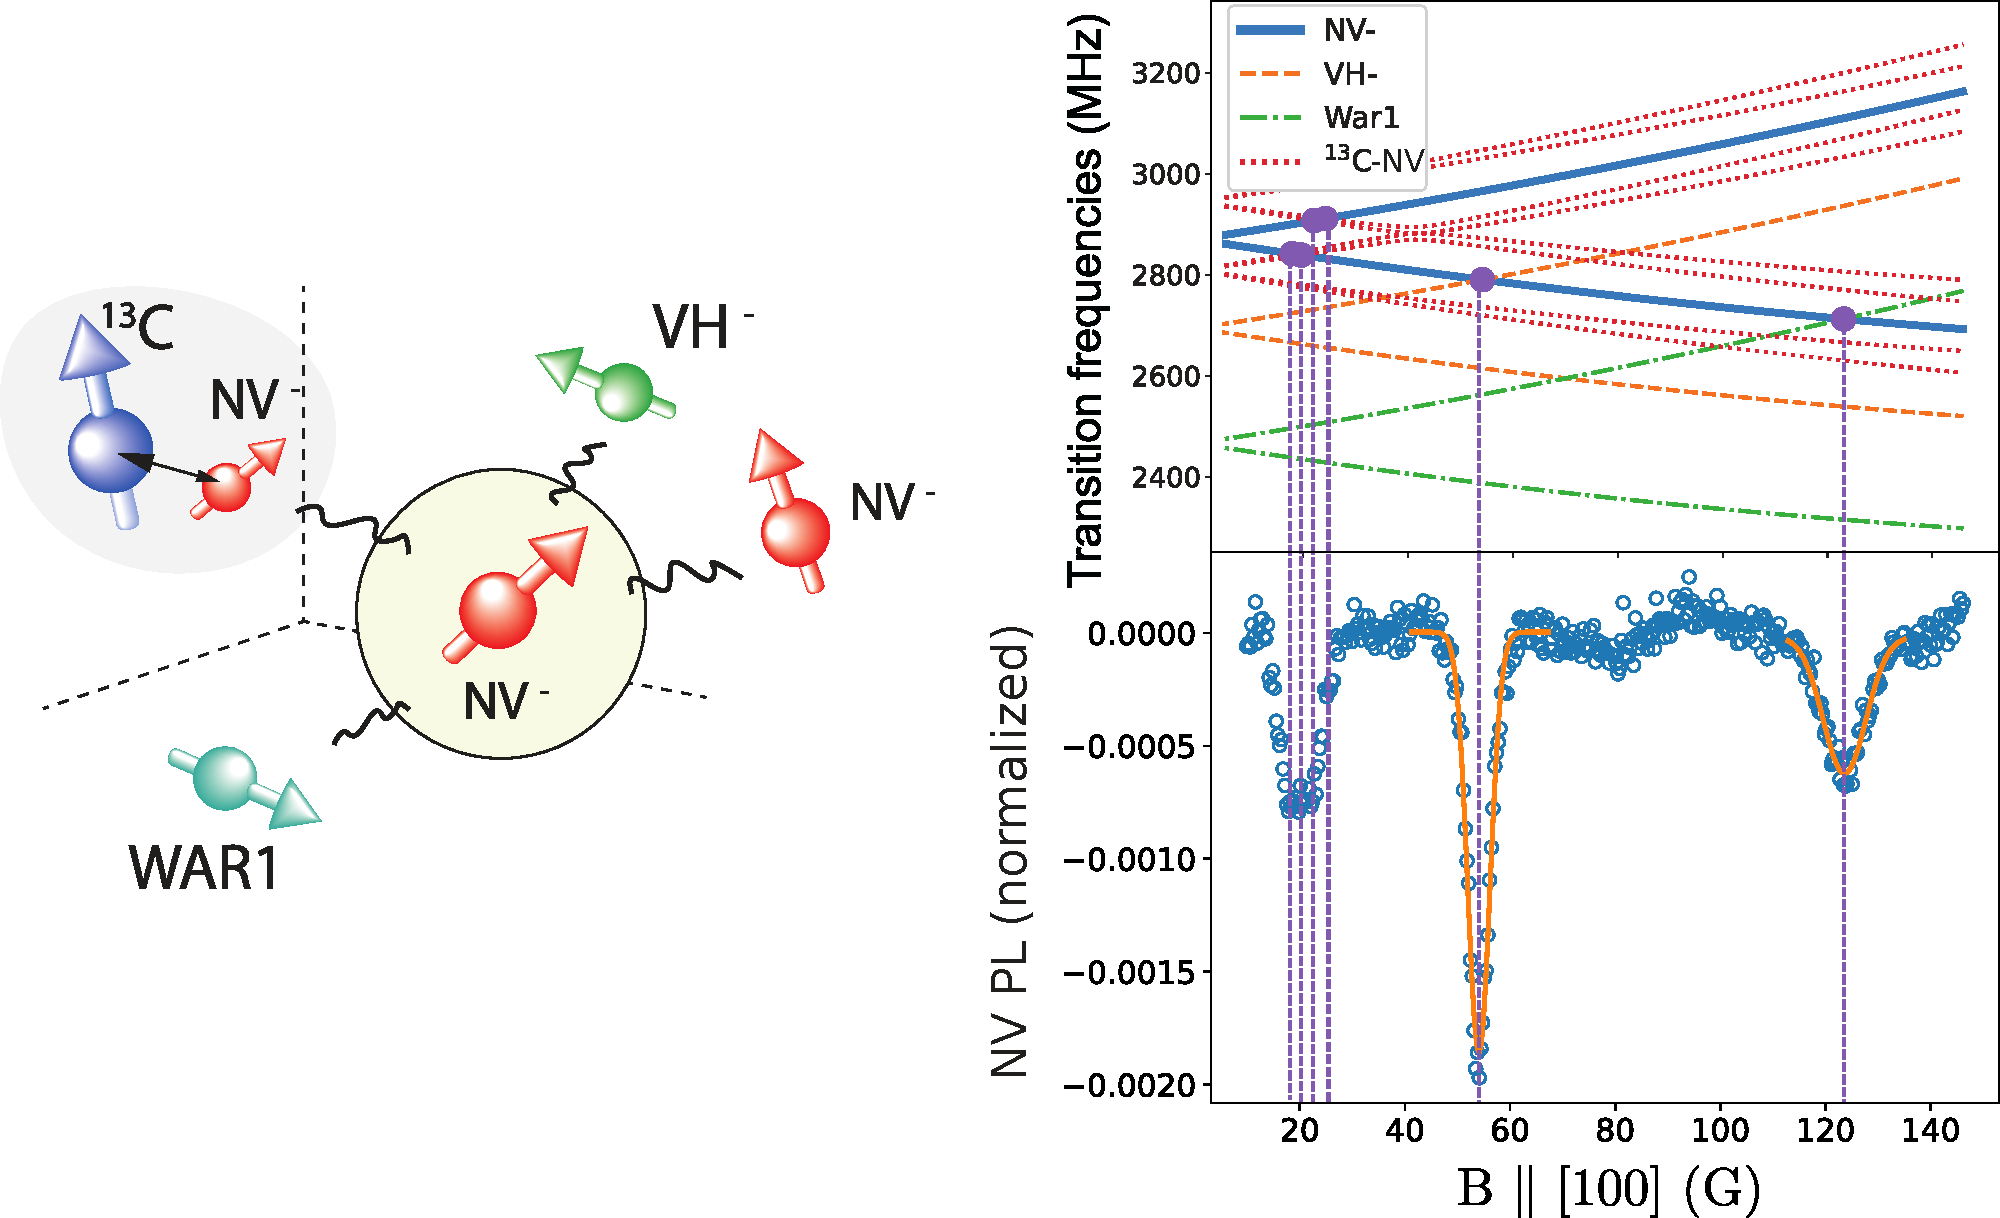
\includegraphics[scale=0.3]{Fig}
\caption{\textbf{I} : Sketch of an NV- center interacting with other spin impurities in diamond.  \textbf{IIa)} Transition energies of the NV center's spin and various dark spins as a function of the external magnetic field. \textbf{IIb)} Normalized photoluminescence of the NV center as a function of the external magnetic field. PL dip lines correspond to resonant interaction between NV centers and other spin impurities in the crystal. \textbf{IIIa)} Lock-in detection of two spin impurities (VH- and War1) for a CVD diamond annealed at 800$^\circ$C. \textbf{IIIb)} Lock-in detection for a similar diamond annealed at 1200$^\circ$C, only the War1 defect remains.}
\end{figure}
\end{abstract}

\maketitle

\begin{thebibliography}{}


\bibitem{Ref2} Pellet-Mary, C., Huillery, P., Perdriat, M., Tallaire, A., Hétet, G. (2021). Physical Review B, 103(10), L100411.

%\bibitem{Ref3} Armstrong, S., Rogers, L. J., McMurtrie, R. L., Manson, N. B. (2010). Physics Procedia, 3(4), 1569-1575.

\bibitem{Ref4} Ngambou, M. W. N., Pellet-Mary, C., Brinza, O., Antonino, A., Hetet, G., Tallaire, A., Bénédic, F. \& Achard, J. (2022).  Diamond and Related Materials, 123, 108884.

\end{thebibliography}
\end{document}
